\documentclass[
% Options for apa7
    a4paper,                % Paper size
    jou,                    % Journal format
    twoside,                % Two-sided printing
    % donotrepeattitle,       % Start body text without repeating title
    floatsintext,           % Insert tables and figures with texts
    biblatex,               % Use BibLaTeX for references
% Options for hyperref
    colorlinks=true,        % Colour all links
    linkcolor=red,          % Cross-references in red
    anchorcolor=black,      % Keep anchors black
    citecolor=blue,         % In-text-referencs in blue
    urlcolor=blue,          % DOIs and URLs are in blue
    bookmarks=true,         % Generate bookmarks for PDF readers
    bookmarksopen=false,    % Expand all bookmarks as default
    bookmarksnumbered=true, % Keep section number in bookmarks
    % Options for xcolor
    dvipsnames              % Use colour BrickRed and PineGreen
]{apa7}

\usepackage{adjustbox}

% Specify absolute path to the tt.sty file, depending on the operating system
\usepackage{ifplatform}
\ifwindows
    \usepackage{M:/pc/Dokumenter/tt}
\fi
\iflinux
    \usepackage{/home/tony/uio/pc/Dokumenter/tt} % Must not use ~ for home directory. Spell in full.
\fi
\ifmacosx
    \usepackage{/Users/tctan/uio/pc/Dokumenter/tt}
\fi

% Specify project's bib library
\addbibresource{./Bibliography/Antisocial.bib}

\setlength\parindent{0.4cm}

\title{Parental Mental Distress and Adolescent Antisocial Behavior:\\
\vspace*{1mm}
The Mediating Role of Family Conflict and Cohesion}
\shorttitle{Family Dynamics and Adolescent Antisocial Behavior}
\leftheader{Skancke, Mausethagen, Tan, {Backer-Gr{\o}ndahl}, \& Bj{\o}rnebekk (2024)}
\journal{\copyright American Psychological Association}
\volume{ISSN: 0033-2909}
\ccoppy{Psychological Bulletin}
\copnum{2024, Vol. 150, No. 2, 91--117\\
\href{https://doi.org/10.1037/bul0000447}{http://dx.doi.org/10.1037/bul0000447}}

\authorsnames[1,1,2,3,{1,3}]{
    Frida T. Skancke,
    Thea Fahle Mausethagen,
    \correspondingauthor{Tony C. A. Tan},\\
    Agathe {Backer-Gr{\o}ndahl},
    Gunnar Bj{\o}rnebekk%
}

\authorsaffiliations{
    {Department of Special Education, University of Oslo},
    {Centre for Educational Measurement, University of Oslo},
    {Norwegian Center for Child Behavioral Development, Oslo, Norway}
}

\authornote{
    \addORCIDlink{Frida T. Skancke}{0000-0002-4374-7038}
    \addORCIDlink{Thea Fahle Mausethagen}{0000-0002-4532-4370}
    \addORCIDlink{Tony C. A. Tan}{0000-0001-6632-3791}
    \addORCIDlink{Agathe {Backer-Gr{\o}ndahl}}{0000-0003-0933-6531}
    \addORCIDlink{Gunnar Bj{\o}rnebekk}{0000-0003-2176-7393}

Correspondence concerning this article should be addressed to Tony Tan, Centre for Educational Measurement, University of Oslo, P.O. Box 1161 Forskningsparken, 0318 Oslo, Norway. E-mail: \href{mailto:tctan@uio.no}{tctan@uio.no}.
}

\abstract{%
Parental mental distress can have a significant impact on adolescents' antisocial behavior (ASB), and this relationship can be exacerbated or alleviated by family dynamics such as conflict and cohesion. By analyzing responses to clinical questionnaires from 157 Norwegian adolescents and their primary caregivers, this study found a significant mediating role family conflict played in strengthening the relationship between parental mental distress and adolescents' ASB. Family cohesion, on the other hand, asserted insufficient protective effect. Both results are consistent with the family stress model, and highlight the importance of addressing not only individuals' mental health but also family-level factors in preventing and treating adolescent ASB. This insight is robust against measurement errors through the use of Bayesian structural equation models.
}

\keywords{%
adolescent antisocial behavior, parental mental distress, family conflict, family cohesion, mediation effect, family stress model, Bayesian structural equation model

\bigskip

\textit{Supplemental materials:} \href{https://doi.org/10.1037/bul0000447.supp}{http://dx.doi.org/10.1037/bul0000447.supp}
}
\begin{document}
\maketitle

\setcounter{page}{91}

%\section{Introduction} % Do not include the word "Introduction" as a Level 1 heading. Just start intro as a normal paragraph immediately after the title.
  % Use \input{} for Intro.tex so that the title and the first paragraph stay on the same page.

% \section{Conceptual Framework}


\subsection{Missing Data Treatment}

IRT item parameter estimations demand strong assumptions on the data missing mechanism. Joint, conditional and marginal maximum likelihood procedures are only valid under ``ignorable non-response'' conditions where missing propensities are related to neither item nor person parameters \parencite{molenaar:1995}. When test takers skip items after seeing their content, for example, the ignorablity condition is unlikely to hold \parencite{mislevy:1987}, neither are tests with items not reached due to time constraint \parencite{lord:1974, lord:1983}. In the current study involving Norway's GPA archive, missing records are not the result of randomly assigning candidates to subjects (not MCAR), nor are each candidate's missing GPAs independent of observed ones (not MAR). In fact, missing patterns are likely to be related to both personal capabilities and subject difficulties with low ability candidates self-selecting into easy subjects while difficult subjects attracting only high capability students. Resultantly, MML estimates of subject difficulties after marginalising personal parameters are no longer unbiased \parencite[][Table 2]{mislevy:1988}.

Literature has congregated into three main approaches for the purpose of addressing missing values. In the \emph{classical approaches}, missing responses can be (a) ignored and treated as non-administered, (b) coded as incorrect, or (c) assigned fractional correct values. This procedure is widely practised amongst international large-scale assessment analysts \parencite{pohl:2014}. Secondly, \emph{imputation-based approaches} encompass corrected mean substitution, response function imputation, EM algorithm and multiple imputation (MI). \textcite{finch:2008} compared the performance of competing imputation-based methods and found MI to be the optimal procedure. MI considers (a) candidates' valid responses, (b) the responses of similar participants, and (c) observed information on covariates if a background model is available, in imputing the missing responses. This Bayesian approach generates multiple draws from parameters' posterior distributions to form correct standard errors \parencite{carpenter:2013}. MI also reallocates the missing-data burden from the analysis stage to the data preparation stage \parencite{reiter:2007}, therefore re-enabling subsequent inferences whose validity depends on complete-data statistical methods and software \parencite[][Chapter 4]{rubin:1987}. Lastly, the recently developed \emph{model-based approaches} include missing tendency in the IRT model when estimating item and person parameters via either (a) latent missing propensity \parencite{holman:2005, glas:2008, glas:2015,korobko:2008} or (b) manifest approach \parencite{rose:2010}.

Both MI and model-based approaches carry their corresponding costs. Studies interested in person parameters shall employ plausible values as the appropriate strategy \parencite{mislevy:1991,mislevy:1993}. But plausible values themselves are multiple imputations of (already multiple imputed) latent variables, causing a cascade of computation demand in the form of nested MI, limiting its wide use in practice such as large-scale assessments or competence tests \parencite{pohl:2014}. Model-based approaches, on the other hand, may generate biased parameter estimates should the missing propensity violate the unidimensionality assumption \parencite{rose:2013}. The current study focuses on \emph{item} parameters (i.e., subject difficulties) while treating person parameters as ``nuisance'' by integrating it out of the maximum likelihood, thereby avoids the MI cascade problem. The risk of committing unidimensionality violation at the missing propensity estimation stage, however, is material since it is not implausible to expect more than one behavioural patterns in young students' GPA choice decisions. It is based on these cost-benefit considerations that this project prefers the MI-based approach to missing data over the model-based procedure.

\section{Methods}

\subsection{Population}

This study retains the entire cohort of Norway's Year 10 students graduating in 2019 as its targeted population. Students' GPA (\textit{grunnskolepoeng}), teacher-assigned grades (\textit{standpunktkarakter}), as well as written (\textit{SKR}) and oral (\textit{MUN}) exam grades were extracted from the national register. This data source is unique because it is the \emph{population}, rather than samples, that forms our unit of analysis. Academic attainment records were then re-shaped into the format that each candidate occupies one row and each subject is represented by one column. This process led to a preliminary data set of 64,918 students and 200 subjects. Next, $4,300$ students without valid GPA records were excluded from subsequent analyses, representing a loss rate of $6.62\%$. Seventeen subjects were retained based on these inclusion criteria:

\subsubsection{Teacher-assigned Grades (12 subjects)}

Under the Norwegian education system, Year 10 students shall complete 13 compulsory subjects as well as electives. This study included all compulsory subjects except for Sidem{\aa}l.\footnote{The Norwegian language has two official written forms: Bokm{\aa}l and Nynorsk, with the former being more prevalent in the media. Students growing up in one written form must enroll the other as their Sidem{\aa}l, unless Norwegian is not their native language. Nynorsk users tend to have easier time in Sidem{\aa}l due to existing exposure to Bokm{\aa}l. Bokm{\aa}l users, on the other hand, find Nynorsk more challenging while fulfilling Sidem{\aa}l. Since Sidem{\aa}l contains two sub-cohorts with distinct difficulty profiles, we opt not to include this subject in our analyses.} We applied equal treatment to courses instructed in Norwegian and in Sami language by merging these records.\footnote{For example, \href{https://www.udir.no/kl06/nat0010}{NAT0010 Naturfag 10. {\aa}rstrinn} and \href{https://www.udir.no/kl06/nat0020}{NAT0020 Naturfag, samisk plan, 10. {\aa}rstrinn} were merged into one subject Natural Sciences. If academic results were available from both instruction languages, we retained the higher grades during merging.} Twelve teacher-assigned grades were included for our analysis: Written Norwegian (NORW), Oral Norwegian (NORO), Written English (ENGW), Oral English (ENGO), Mathematics (MATH), Natural Sciences (NATS), Social Sciences (SOCS), Religion (RELI), Music (MUSI), Arts and Handcraft (HAND), Food and Health (FOOD), and Physical Education (PHED).

\subsubsection{Written Exam Grades (3 subjects)}

Norway uses a lottery draw to randomly assign Year 10 students to participate in \emph{one} of the following three written exams: Norwegian (E-NORW), English (E-ENGW) and mathematics (E-MATH). This ``planned missingness'' implies that although numeral in quantity, the unobserved exam grades can be safely modelled under the missing completely at random (MCAR) assumption \parencite{little:2019}.\footnote{Even if the lottery is less than perfectly random, Rasch models are still valid under the weaker assumption of missing at random (MAR), as long as one is satisfied that missing propensities are unrelated to item or person parameters \parencite{molenaar:1995}.} Rasch models have a major advantage for handling missing values thanks to the sufficient overlap across subjects in the score matrix \parencite{he:2018}.

\subsubsection{Oral Exam Grades (2 subjects)}

Year 10's oral exams consist of the same three subjects as in written exams, plus a wide selection such as natural and social sciences, with students being randomly assigned into \emph{one} oral exam by lottery. In order to better match teacher-assigned grades, only Oral Norwegian (E-NORO) and Oral English (E-ENGO) were included in this study. Since students are spread thinly across many oral exam subjects, E-NORO and E-ENGO appeared more sparse than their teacher-assigned counterparts, leading to larger confidence intervals in subsequent analyses.


\section{Results}

\subsection{Descriptive Statistics}

\cref{tab:descriptive} summarised key information about the 18 \textsc{gpa} subjects examined by this study, including the number of valid entries, grade distributions, and links to official documentation. It is firstly noticeable that data missing rates differed significantly across modes of assessment. Teacher-assigned grades carried small missing percentages most under 5 percent, hence imposing little concerns over estimation bias. Although written- and oral-exams had large missing percentages, this was the effect of the equal-probability sampling procedures. Under planned missingness, the observed grades represent unbiased estimates of true grades despite only 1/3 or 1/5 of the students were studied.

Secondly, grade distributions differed both between- and within-modes of assessment. A large number of grade counts clustered around Grade 3 and 4 for external exams, whereas teacher-assigned grades peaked at different bands depending on the subject, with \textsc{math} mainly covering Grade 2 to 4 while \textsc{food} covering largely Grade 4 and 5.

\subsection{Subject Difficulties}

\subsubsection{Overall Difficulties}
\textsc{gpa} subjects' overall difficulties are shown in \cref{fig:expected}. Using \textsc{math} as an example, the horizontal axis of Panel A represents students' latent competencies, ranging from low ($\theta=-10$) to high ($\theta=5$), and the vertical axis represents grades randing from $1$ to $6$. Students with low competencies are expected to receive Grade 1 while Grade 6 is reserved to students with very high competencies. Mapping every competency level to its expected grade yields the sigmoid curve in Panel A. Furthermore, there exists a median student, who evenly divides \textsc{math}'s observations into 50\% below, and 50\% above him/her, whose $\theta$ is defined as zero. Tracing this median student's expected score from the curve in Panel A, one reads a grade of 3.64 as the \emph{overall difficulty} for \textsc{math}. Repeating this procedure for all 18 GPA subjects gave rise to the scatter plot in Panel B. Subject with low expected grades such as \textsc{math} are more difficult while \textsc{phed} and \textsc{food} are easy subjects evidenced by the high expected grades from median students.

Ranked by overall difficulties, teacher-assigned grades appeared to align themselves along the \textit{manu}--\textit{mente} dichotomy. A median student is expected to receive a score one grade lower in the most difficult subject \textsc{math} than from the easiest one \textsc{phed}. Written exams are more difficult than oral exams, with \textsc{nor\_w} being more difficult than teacher-assigned \textsc{math}. Oral English exam, in contrast, is comparable in difficulty to \textit{mente} subjects such as teacher-assigned \textsc{food}.

\subsubsection{Grade-level Difficulties}
This study operationalises grade-level difficulties using difficulty thresholds. For a polytomous \textsc{irt} item such as \textsc{math}, a category characteristic curve (\textsc{ccc}) describes the likelihood a particular grade is received by students with varying competency levels. The $P1$ curve in Panel A \cref{fig:grade_level}, for example, states that Grade 1 is awarded to students with low competencies almost surely (probability approaching 1) but to those with high competencies almost never (probability approaching 0). Similarly, the $P2$ curve suggests that Grade 2 is most likely to be awarded to students with competencies between approximately $\theta=[-6, -1]$ but low probabilities outside this domain. The intersection between $P1$ and $P2$ marks a difficulty threshold $\delta_1$, above which the next grade is more likely. Six \textsc{ccc}s produce five difficulty thresholds $\delta_1, \dots, \delta_5$, which concisely summarise each subject's \emph{grade-level difficulties}. Repeating this procedure to all 18 \textsc{gpa} subjects produces Panel B.

Among teacher-assigned grades, the competency demands for receiving a particular grade differed widely depending on the low- and high-end of the grading scale. High consistency was observed at the $\delta_5$-level where all subjects required students to have high competencies ($\theta \approx 2.5$) to transitions from Grade 5 to the top grade 6. As one moves down the grade ladder, however, the difficulty gap expanded to more than one grade between the most difficult subject and the easiest one such that a Grade 3 in \textsc{math} is more comparable to a Grade 4 in \textsc{food}. Lastly, the lengthening 95\% confidence intervals in $\delta_1$ suggests that teachers did not fully utilise the entire grade scale, especially for the \textit{manu} subjects---an observation corroborated by the grade distributions in \cref{tab:descriptive}.

\subsection{Model Fit Measures and Information Curves}

\cref{fig:fit} visualises the Rasch model fit statistics using the 2019 Year 10 \textsc{gpa} data. A model with perfect fit would generate an information weighted fit (infit) and unweighted fit mean square (outfit) of $1$ \parencite{wu:2016}. Infit and outfit mean squares below $1$ suggest overfit where the item is more discriminating than the average item discrimination. Resultantly, \textcite{wu:2016} consider high quality items (\textit{mente} subjects) to have mean squares less than $1$ even though some of these items may be deemed as misfitting the model. \textsc{gpa} subjects with mean squares much greater than $1$ are deemed poorer \textsc{irt} items. Under these criteria, teacher-assigned grades for \textit{manu} subjects \textsc{hand}, and \textsc{phed} showed poor model fit, as well as oral English exam grades.

Lastly, \cref{fig:info} presents the information curves (left scale, blue) for the 18 \textsc{gpa} subjects. An information curve plots the information function against the latent competency. The information function is the expected information gained from a student's response to an item given their competency level. \cref{fig:info} also displays the standard error curves (right scale, red) that communicate the precision of each Rasch item over the competency range. The information and standard error curves jointly suggest that the Rasch model used in this study provided strong explanatory power and high precision over the mid-range of the latent competency scale where most students reside.


\section{Discussion}

The purpose of this current study was to investigate whether family conflict and cohesion have a mediating role on the relationship between parental mental distress (PMD) and adolescent antisocial behavior (ASB). Results revealed a direct association between PMD and adolescent ASB, and is consistent with previous research. Indicating that PMD with all the possible behaviors or attitudes this measure includes, directly affects adolescents development and exhibition of ASB. Some mechanisms that might influence, but are not controlled for in the current study include parenting styles \parencite{hautmann:2015, vera:2012}, parental hostility and overprotection \parencite{sellers:2014}, and coping strategies \parencite{francisco:2015}, as well as environmental factors outside the family (KILDE). Further, our overall results indicate that family conflict has a mediating effect on adolescent ASB, while cohesion does not. Unsurprisingly, elevated and chronic patterns of family conflict, and within specific dyads, e.g. parent-adolescent, results in deteriorated family cohesion.

As to our first hypothesis, results indicate that elevated levels of PMD is associated with increased levels of family conflict, and reduction in family cohesion. These results are consistent with previous findings \parencite[e.g.,][]{garber:2005, perez:2018, xu:2017}. We assume that PMD negatively affects their ability to choose proactive and effective parenting strategies, as previous research has found that depressed caregivers use inconsistent discipline, initiate negative patterns of interactions, and lack monitoring \parencite{korhonen:2014,perez:2018}. Factors like these are possible explanations for why family environments with distressed caregivers may function as catalysts for adverse interaction patterns, resulting in chronic conflict-filled communication between family members \parencite{garber:2005}.  Hostile and conflict-filled interpersonal relationships can result in withdrawal by family members \parencite{romm:2022}. Hence, explaining the reduction in family cohesion when PMD is high. These results are also in line with previous research \parencite{li:2021, vanloon:2014}. It is reasonable to assume that within a clinical sample, with interactions characterized by higher conflict and PMD, any deterioration in family cohesion will escalate the situation.

As expected, results indicate that family conflict has a mediating role on the relationship between PMD and adolescent ASB, while cohesion does not. There are several explanations for why and how family conflict has an impact on the path to adolescent ASB. Parents with increased mental distress usually have reduced capacity and ability to engage in positive and favorable parenting \parencite{joyner:2021}. As depression and anxiety influence parenting styles characterized by control through guilt and overprotection, hostility, criticism, and inconsistent discipline \parencite{cummings:2005,korhonen:2014}. This may result in family environments characterized by coercive and hostile attitudes and behaviors. \textcite{lobraico:2020} found that adolescents in coercive families experienced the most robust risk across ASB outcomes. Families that engage in more hostile behaviors, in the form of fighting and aggression, may damage both trust and secure attachments between parent and adolescent \parencite{buehler:2006,weymouth:2016}. When this pattern of communication becomes normative within the family, offsprings may adopt and stabilize these attitudes to other social relations, encouraging affiliation with antisocial groups and peers \parencite{carroll:2009,ciranka:2021,moffitt:2015}. Conversely, research shows that living with antisocial or delinquent adolescents have transactional adverse consequences on PMD and family conflict \parencite{gross:2009}. For instance, having a teen not complying to rules, expressing hostile and aggressive behaviors, and parents' awareness that they engage in antisocial activities may create significant stress \parencite{allen:2010}.

Adolescence brings normative shifts in family relations, resulting in increased conflict and reduced cohesion between parent and youth, as they attempt to adjust boundaries, renegotiate parental authority, and increase their autonomy and independence \parencite{baer:2002,lin:2019,weymouth:2016}. Youth also tend to become more oppositional during adolescence \parencite{steinberg:2011}, which may exacerbate adverse patterns of communication and interaction. Also, parents modeling role on behaviors and attitudes are gradually replaced by peers. Developmental trends like these become more problematic for mentally distressed parents, compared to non-distressed. We assume that PMD might exacerbate their ability to meet and adjust to adolescent autonomy seeking, resulting in even more friction and conflict. Connectedness and youth self-disclosure are found to significantly enhance youths' prosperity to seek guidance when navigating difficulties, value parental input, and spend time with their families. Hence, leaving them with less opportunity to engage in ASB \parencite{ackard:2006,crawford:2008,vieno:2009}. Therefore, we assume that high conflict and lack of cohesion in our sample, contribute to the youth seeking affiliation with deviant peers and not their parents. Especially among mentally distressed parents, where rejection and love withdrawal are prominent. This may exacerbate the distance between parent and adolescent.

When controlling for economic hardship, we found that this had an influence on PMD and family conflict, but not on adolescent ASB. These findings suggest that economic hardship directly impacts parents. Previous research has found socioeconomic disadvantage to be a strong indicator of depressive symptoms in parents \parencite{conger:2010,sturgeapple:2014,vreeland:2019}. Therefore, we assume that living in economic disadvantage might place the parents under elevated stress, which further impair their parental practices and family climate. Further, PMD may also be a contributing factor to poorer employability, therefore more economic hardship. Resultantly, this stressor may be a reason for increased levels of family conflict within the family system, and have an indirect influence on adolescent ASB.

\subsection{Limitations}

This study has several limitations. Firstly, a consequence of small sample size is lack of power to detect statistical significance for the observed associations. Secondly, we only used parent-reported measures. This is problematic due to well documented discrepancies between parental and adolescents' reports on family environment and ASB \parencite[e.g.,][]{delosreyes:2011, robinson:2019}, introducing a potential reporting bias (Allen et al., 2010). Parents and adolescents may interpret and observe each other's behaviors differently, therefore, research should attempt to include the offspring's perspectives. Further, cross-sectional data prevents us from drawing any causal conclusions. Our findings are an artifact of our modelling choices, reflecting that results could be different using other methods and samples. For example, compared to the general population, a clinical sample usually has higher levels of symptoms, with in turn affects the generalization of our findings. The current study provides a small ``snapshot'' of a bigger picture. However, this still contributes to research, as many small ``snapshots'' jointly inform the full picture.

\subsection{Implications and Future Research}

Findings from the current study have various practical implications. This study provides insight and confirmation of previous research on the association between family mechanisms, PMD and adolescent ASB. This is important when establishing holistic interventions, targeting environmental factors and parents' psychopathology. Results suggest that family interaction patterns, such as conflict and cohesion, have significant and distinct influences on interpersonal relationships, feelings and behaviors among family members. Further research should seek to use multi-informants, youths' perspectives, and differentiate by gender when examining relations between interpersonal and environmental constructs.


\subsection{Data Availability}

\subsection{Acknowledgments}

\subsection{Author Contributions}

\subsection{Ethical Considerations}

To ensure acceptable principles of ethical and professional conduct, the current study received approval from Regional Committees for Medical and Health Research Ethics (REK) to utilize data gathered by the study of Evaluation of Functional Family Therapy in Norway \parencite{bjornebekk:2013}. All participants, both parents and adolescents gave written informed consent. Consent forms included information about participants' right to withdraw from the study at any given time, and ensured participants confidentiality. Participants consent forms were presented for Norwegian Center for Research Data (NSD) and Norwegian Data Protection Authority [Datatilsynet] \parencite{bjornebekk:2013}. All data were collected, stored, and processed within a certified secure IT environment \parencite[TSD,][]{tsd:2020}.

\printbibliography

% Figures
\onecolumn
\ttptikz{fig:bayes}{Structural Equation Model Predicting Youth's Antisocial Behavior}{
\begin{tikzpicture}[
    manvar/.style={rectangle,draw=black,minimum width=1.5cm},
    latvar/.style={ellipse,draw=black,minimum width=1.5cm,minimum height=1cm},
    convar/.style={rectangle,draw=black!25!white,minimum width=1.5cm},
    mean/.style={fill=black!10!white,regular polygon,regular polygon sides=3},
    ->,>=stealth',semithick,
    bend angle=-45,
    decoration={
        zigzag,
        amplitude=1pt,
        segment length=1mm,
        post=lineto,
        post length=4pt
    }
]

% Set parental mental health (input variable, X)
\node[latvar] (X) at (0,0) {PMH};

% Set family conflict and family cohesion (mediators, M)
\node[latvar] (M1) at (5,2.5) {CON};
\node[latvar] (M2) at (5,-2.5) {COH};

% Set antisocial behaviour (outcome variable, Y)
\node[latvar] (Y) at (13,0) {ASB};

% Link X to M
\draw[->,line width=2*0.500mm] (X.east) to node[above,sloped] {\press{0.502}{***}{0.074}} (M1.west);
\draw[->,line width=2*0.434mm] (X.east) to node[above,sloped] {\press{-0.434}{***}{0.080}} (M2.west);

% Lind M to Y
\draw[->,line width=2*0.512mm] (M1.east) to node[above,sloped] {\press{0.512}{**}{0.143}} (Y.west);
\draw[->,dashed] (M2.east) to (Y.west);

% Link X to Y
\draw[->,line width=2*0.347mm] (X.east) to node[above,pos=0.72] {\press{0.347}{***}{0.108}} (Y.west);

% Covariance between M1 and M2
\draw[black!25!white,<->,line width=2*0.530mm] (M1.south) to [bend right] (M2.north);

% Control variable (HAR)
\node[manvar] (S) at (13,-2.5) {HAR};

% Link SES to Y
\draw[->,line width=2*0.210mm] (S.north) to node[above,sloped] {\press{-0.210}{**}{0.083}} (Y.south);

\end{tikzpicture}
}{This structural equation model predicts youth's antisocial/externalizing behavior (ASB) from parental mental health (PMH), with mediating effects from family conflict (CON) and family cohesion (COH). Variables in ellipses are latent constructs (see \cref{app:latent}). Standardized regression coefficients are computed using Bayes estimator \parencite{depaoli:2021} and averaged over ten imputed datasets \parencite{little:2020, vanbuuren:2018}. Solid lines are visualized in proportion to their estimates while dashed lines represent nonsignificant relations at $\alpha=.05$ level. Parental perception of economic hardship (HAR) is only significantly related to the outcome variable ASB. All control variables are nonsignificant and are omitted from the diagram.\\
    $^* p < .05$. $^{**} p < .01$. $^{***} p < .001$.
}

% Tables

\ttptable{tab:demographic}{Socio-demographic Characteristics of Participants}{
    \begin{tabular}{lrcc}
        \toprule
        \multicolumn{1}{c}{Sample Characteristics} & \multicolumn{1}{c}{$n$} & \multicolumn{1}{c}{$M$ ($SD$)} & \multicolumn{1}{c}{Missing} \\
        \midrule
        \rowcolor[rgb]{ .949,  .949,  .949} Adolescents' Age & 157   & 14.74 (1.47) &  \\
        \rowcolor[rgb]{ .949,  .949,  .949} Adolescents' Gender & 157   &       &  \\
        \hspace{0.75cm} Female & 72    &       &  \\
        \hspace{0.75cm} Male & 85    &       &  \\
        \rowcolor[rgb]{ .949,  .949,  .949} Adolescents' Living Condition & 153   &       & 2.50\% \\
        \hspace{0.75cm} Category 1: Living at home with their parents & 40    &       &  \\
        \hspace{0.75cm} Category 2: Living partly with both parents & 8     &       &  \\
        \hspace{0.75cm} Category 3: Living mainly with one parent who have no new partner & 59    &       &  \\
        \hspace{0.75cm} Category 4: Living mainly with one parent who has a new partner & 36    &       &  \\
        \hspace{0.75cm} Category 5: Being adopted or living in foster care & 10    &       &  \\
        &&&\\
        \rowcolor[rgb]{ .949,  .949,  .949} Parental Age & 157   & 43.9 (6.90) &  \\
        \rowcolor[rgb]{ .949,  .949,  .949} Parental Gender & 157   &       &  \\
        \hspace{0.75cm} Mother & 141   &       &  \\
        \hspace{0.75cm} Father & 16    &       &  \\
        \rowcolor[rgb]{ .949,  .949,  .949} Parental Education Level & 156   &       & 0.60\% \\
        \hspace{0.75cm} Level 1: Primary and secondary school (< 10 years) & 23    &       &  \\
        \hspace{0.75cm} Level 2: Upper secondary school (11--14 years) & 67    &       &  \\
        \hspace{0.75cm} Level 3: Higher education (> 14  year) & 66    &       &  \\
        \rowcolor[rgb]{ .949,  .949,  .949} Perceived Economic Hardship & 156   &       & 0.60\% \\
        \hspace{0.75cm} Level 1: Living comfortably & 12    &       &  \\
        \hspace{0.75cm} Level 2: Doing alright & 43    &       &  \\
        \hspace{0.75cm} Level 3: Just about getting it & 76    &       &  \\
        \hspace{0.75cm} Level 4: Finding it quite difficult & 15    &       &  \\
        \hspace{0.75cm} Level 5: Finding it very difficult & 10    &       &  \\
        &&&\\
        \rowcolor[rgb]{ .949,  .949,  .949} Additional Children in the Family & 157   & 1.25 (0.99) &  \\
        \bottomrule
    \end{tabular}%
}{Categorical variables are coded using their category/level numbers. The means ($M$) and standard deviations ($SD$) of non-categorical variables are measured in their natural units (e.g., years of age).}


\ttltable{tab:descriptive}{Descriptive Statistics for the 18 GPA Subjects}{
    \begin{tabular}{clrrrrrrrrrl}
        \toprule
    Subject & \multicolumn{1}{c}{Subject} & \multicolumn{1}{c}{Valid} & \multicolumn{1}{c}{Missing} & \multicolumn{1}{c}{Missing} & \multicolumn{6}{c}{Grade Frequency}           & \multicolumn{1}{c}{\textsc{udir}} \\
    \cmidrule{6-11}    Code  & \multicolumn{1}{c}{Name} & \multicolumn{1}{c}{Entries} & \multicolumn{1}{c}{($n$)} & \multicolumn{1}{c}{($\%$)} & \multicolumn{1}{c}{1} & \multicolumn{1}{c}{2} & \multicolumn{1}{c}{3} & \multicolumn{1}{c}{4} & \multicolumn{1}{c}{5} & \multicolumn{1}{c}{6} & \multicolumn{1}{c}{Course Code} \\
        \midrule
        \multicolumn{12}{l}{\textbf{Teacher-assigned Grades} (12 subjects)}\\
    \textsc{math}  & Mathematics & 59,184 & 1,434 & 2.37  & 1,165 & 10,086 & 15,447 & 15,443 & 12,520 & 4,523 & \href{https://www.udir.no/lk20/fagkoder/mat0010}{\textsc{mat0010}} \\
    \textsc{norw}  & Written Norwegian & 58,946 & 1,672 & 2.76  & 498   & 5,504 & 15,503 & 20,482 & 13,888 & 3,071 & \href{https://www.udir.no/lk20/fagkoder/nor0214}{\textsc{nor0214}} \& \href{https://www.udir.no/lk20/fagkoder/nor0041}{\textsc{nor0041}} \\
    \textsc{engw}  & Written English & 59,047 & 1,571 & 2.59  & 850   & 5,315 & 13,671 & 19,934 & 14,937 & 4,440 & \href{https://www.udir.no/lk20/fagkoder/eng0012}{\textsc{eng0012}} \\
    \textsc{nats}  & Natural Sciences & 59,642 & 976   & 1.61  & 490   & 4,801 & 12,134 & 17,179 & 17,448 & 7,590 & \href{https://www.udir.no/lk20/fagkoder/nat0010}{\textsc{nat0010}} \& \href{https://www.udir.no/lk20/fagkoder/nat0020}{\textsc{nat0020}} \\
    \textsc{noro}  & Oral Norwegian & 58,982 & 1,636 & 2.70  & 210   & 2,994 & 10,855 & 18,764 & 19,254 & 6,905 & \href{https://www.udir.no/lk20/fagkoder/nor0216}{\textsc{nor0216}} \& \href{https://www.udir.no/lk20/fagkoder/nor0042}{\textsc{nor0042}} \\
    \textsc{engo}  & Oral English & 59,148 & 1,470 & 2.43  & 441   & 3,200 & 9,938 & 19,725 & 18,947 & 6,897 & \href{https://www.udir.no/lk20/fagkoder/eng0013}{\textsc{eng0013}} \\
    \textsc{reli}  & Religion & 56,993 & 3,625 & 5.98  & 316   & 3,386 & 9,928 & 16,966 & 18,293 & 8,104 & \href{https://www.udir.no/lk20/fagkoder/RLE0030}{\textsc{rle0030}} \& \href{https://www.udir.no/lk20/fagkoder/rel0040}{\textsc{rel0040}} \\
    \textsc{socs}  & Social Sciences & 59,715 & 903   & 1.49  & 307   & 3,466 & 10,489 & 17,527 & 19,538 & 8,388 & \href{https://www.udir.no/lk20/fagkoder/saf0010}{\textsc{saf0010}} \& \href{https://www.udir.no/lk20/fagkoder/saf0020}{\textsc{saf0020}} \\
    \textsc{musi}  & Music & 57,716 & 2,902 & 4.79  & 120   & 1,450 & 6,771 & 18,830 & 22,940 & 7,605 & \href{https://www.udir.no/lk20/fagkoder/mus0010}{\textsc{mus0010}} \& \href{https://www.udir.no/lk20/fagkoder/mus0020}{\textsc{mus0020}} \\
    \textsc{hand}  & Arts and Handcraft & 58,001 & 2,617 & 4.32  & 93    & 1,142 & 6,876 & 19,744 & 23,140 & 7,006 & \href{https://www.udir.no/lk20/fagkoder/khv0010}{\textsc{khv0010}} \& \href{https://www.udir.no/lk20/fagkoder/khv0020}{\textsc{khv0020}} \\
    \textsc{phed}  & Physical Education & 57,731 & 2,887 & 4.76  & 102   & 913   & 4,612 & 16,606 & 26,037 & 9,461 & \href{https://www.udir.no/lk20/fagkoder/kro0020}{\textsc{kro0020}} \\
    \textsc{food}  & Food and Health & 57,683 & 2,935 & 4.84  & 16    & 561   & 6,060 & 19,098 & 23,907 & 8,041 & \href{https://www.udir.no/lk20/fagkoder/mhe0010}{\textsc{mhe0010}} \& \href{https://www.udir.no/lk20/fagkoder/mhe0020}{\textsc{mhe0020}} \\
        \multicolumn{12}{l}{\textbf{Written Exam Grades} (3 subjects)}\\
    \textsc{mat\_w} & Written Mathematics & 15,252 & 45,366 & 74.84 & 235   & 2,482 & 4,261 & 4,529 & 2,902 & 843   & \href{https://www.udir.no/lk20/fagkoder/mat0010}{\textsc{mat0010}} \\
    \textsc{nor\_w} & Written Norwegian & 13,851 & 46,767 & 77.15 & 237   & 2,345 & 5,245 & 4,106 & 1,616 & 302   & \href{https://www.udir.no/lk20/fagkoder/nor0214}{\textsc{nor0214}} \\
    \textsc{eng\_w} & Written English & 14,723 & 45,895 & 75.71 & 225   & 1,573 & 4,224 & 4,940 & 2,913 & 848   & \href{https://www.udir.no/lk20/fagkoder/eng0012}{\textsc{eng0012}} \\
        \multicolumn{12}{l}{\textbf{Oral Exam Grades} (3 subjects)}\\
    \textsc{mat\_o} & Oral Mathematics & 8,838 & 51,780 & 85.42 & 16    & 770   & 2,041 & 2,503 & 1,958 & 1,550 & \href{https://www.udir.no/lk20/fagkoder/mat0011}{\textsc{mat0011}} \\
    \textsc{nor\_o} & Oral Norwegian & 9,310 & 51,308 & 84.64 & 34    & 459   & 1,651 & 2,520 & 2,342 & 2,304 & \href{https://www.udir.no/lk20/fagkoder/nor0216}{\textsc{nor0216}} \\
    \textsc{eng\_o} & Oral English & 9,207 & 51,411 & 84.81 & 36    & 330   & 1,405 & 2,651 & 2,452 & 2,333 & \href{https://www.udir.no/lk20/fagkoder/eng0013}{\textsc{eng0013}} \\
        \bottomrule
    \end{tabular}%
}{
    Missing counts ($n$) and percentages ($\%$) were computed relative to the population size $N = 60,618$. Official documentation about each subject is available from the Norwegian Ministry of Education (\textsc{udir}) database by clicking each hyperlink. Subjects offered in both Norwegian and Sami as instruction languages are merged, with both codes given in the \textsc{udir} column.
}

\ttltable{tab:descriptive}{Variance-covariance Matrix and Correlation Table of Key Variables}{
      \begin{tabular}{clrrrrrrrrr}
      \toprule
      Seq   & \multicolumn{1}{c}{Variable} & \multicolumn{1}{c}{1} & \multicolumn{1}{c}{2} & \multicolumn{1}{c}{3} & \multicolumn{1}{c}{4} & \multicolumn{1}{c}{5} & \multicolumn{1}{c}{6} & \multicolumn{1}{c}{7} & \multicolumn{1}{c}{8} & \multicolumn{1}{c}{9} \\
      \midrule
      1     & YAGE  & \textbf{2.152} & \cellcolor[rgb]{ .745,  .745,  1}0.257 & \cellcolor[rgb]{ 1,  .851,  .851}$-$0.146 & \cellcolor[rgb]{ .902,  .902,  1}0.101 & \cellcolor[rgb]{ 1,  .984,  .984}$-$0.013 & \cellcolor[rgb]{ 1,  .906,  .906}$-$0.091 & \cellcolor[rgb]{ .863,  .863,  1}0.140 & \cellcolor[rgb]{ .965,  .965,  1}0.038 & \cellcolor[rgb]{ 1,  .996,  .996}$-$0.003 \\
      2     & PAGE  & 2.599 & \textbf{47.365} & \cellcolor[rgb]{ 1,  .686,  .686}$-$0.310 & \cellcolor[rgb]{ .776,  .776,  1}0.226 & \cellcolor[rgb]{ 1,  .898,  .898}$-$0.101 & \cellcolor[rgb]{ .949,  .949,  1}0.054 & \cellcolor[rgb]{ .918,  .918,  1}0.083 & \cellcolor[rgb]{ 1,  .918,  .918}$-$0.079 & \cellcolor[rgb]{ 1,  .949,  .949}$-$0.050 \\
      3     & SIB   & $-$0.214 & $-$2.122 & \textbf{0.992} & \cellcolor[rgb]{ 1,  .945,  .945}$-$0.052 & \cellcolor[rgb]{ .992,  .992,  1}0.009 & \cellcolor[rgb]{ .996,  .996,  1}0.005 & \cellcolor[rgb]{ 1,  .996,  .996}$-$0.002 & \cellcolor[rgb]{ .898,  .898,  1}0.105 & \cellcolor[rgb]{ 1,  .992,  .992}$-$0.004 \\
      4     & INC   & 33.367 & 348.795 & $-$11.532 & \textbf{50,467.613} & \cellcolor[rgb]{ 1,  .933,  .933}$-$0.065 & \cellcolor[rgb]{ .992,  .992,  1}0.010 & \cellcolor[rgb]{ 1,  .914,  .914}$-$0.083 & \cellcolor[rgb]{ .973,  .973,  1}0.030 & \cellcolor[rgb]{ 1,  .588,  .588}$-$0.411 \\
      5     & PMH\_SUM & $-$0.095 & $-$3.593 & 0.046 & $-$75.449 & \textbf{26.738} & \cellcolor[rgb]{ .588,  .588,  1}0.414 & \cellcolor[rgb]{ 1,  .694,  .694}$-$0.302 & \cellcolor[rgb]{ .6,  .6,  1}0.403 & \cellcolor[rgb]{ .831,  .831,  1}0.171 \\
      6     & CON\_SUM & $-$0.319 & 0.886 & 0.011 & 5.111 & 5.110  & \textbf{5.697} & \cellcolor[rgb]{ 1,  .541,  .541}$-$0.455 & \cellcolor[rgb]{ .608,  .608,  1}0.396 & \cellcolor[rgb]{ .804,  .804,  1}0.199 \\
      7     & COH\_SUM & 0.476 & 1.322 & $-$0.004 & $-$43.410 & $-$3.614 & $-$2.515 & \textbf{5.367} & \cellcolor[rgb]{ 1,  .741,  .741}$-$0.258 & \cellcolor[rgb]{ 1,  .937,  .937}$-$0.062 \\
      8     & ASB\_SUM & 0.698 & $-$6.793 & 1.307 & 84.089 & 25.908 & 11.768 & $-$7.447 & \textbf{154.805} & \cellcolor[rgb]{ 1,  .957,  .957}$-$0.041 \\
      9     & HAR   & $-$0.004 & $-$0.327 & $-$0.003 & $-$87.556 & 0.839 & 0.449 & $-$0.135 & $-$0.481 & \textbf{0.898} \\
      \phantom{9} & \phantom{PMH\_SUM} & \phantom{50,467.613} & \phantom{50,467.613} & \phantom{50,467.613} & \phantom{50,467.613} & \phantom{50,467.613} & \phantom{50,467.613} & \phantom{50,467.613} & \phantom{50,467.613} & \phantom{50,467.613}\\
      \bottomrule
      \end{tabular}
}{This table summarizes variables' variances (diagonal elements, bold), their covariances (lower triangle) and correlations (upper triangle, with heat map).}


\ttptable{tab:lat_PMH}{Confirmatory Factor Analysis for Latent Construct Parental Mental Health (PMH)}{
    \begin{tabular}{cc c rrrr c rr@{\hskip -0.08mm}l c c}
    \toprule
    \multicolumn{2}{c}{Item} &       & \multicolumn{4}{c}{Category Count} &       & \multicolumn{3}{c}{Factor Loading}       &       & \multicolumn{1}{c}{Residual} \\
\cmidrule{1-2}\cmidrule{4-7}\cmidrule{9-11}    Seq   & Code  &       & \multicolumn{1}{c}{1} & \multicolumn{1}{c}{2} & \multicolumn{1}{c}{3} & \multicolumn{1}{c}{4} &       & \multicolumn{1}{c}{$\lambda$} & \multicolumn{2}{c}{$SE(\lambda$)}       &       & \multicolumn{1}{c}{Variance} \\
    \midrule
    1     & SCL8\_01 &       & 70    & 60    & 19    & 7     &       & 0.872 & 0.026 & $^{***}$   &       & 0.046 \\
    2     & SCL8\_02 &       & 69    & 60    & 22    & 5     &       & 0.891 & 0.028 & $^{***}$   &       & 0.049 \\
    3     & SCL8\_03 &       & 48    & 67    & 29    & 12    &       & 0.849 & 0.029 & $^{***}$   &       & 0.049 \\
    4     & SCL8\_04 &       & 68    & 58    & 24    & 6     &       & 0.862 & 0.030 & $^{***}$   &       & 0.053 \\
    5     & SCL8\_05 &       & 32    & 77    & 35    & 12    &       & 0.825 & 0.029 & $^{***}$   &       & 0.047 \\
    6     & SCL8\_06 &       & 45    & 67    & 33    & 11    &       & 0.773 & 0.037 & $^{***}$   &       & 0.053 \\
    7     & SCL8\_07 &       & 66    & 57    & 26    & 7     &       & 0.716 & 0.043 & $^{***}$   &       & 0.062 \\
    8     & SCL8\_08 &       & 130   & 21    & 2     & 3     &       & 0.515 & 0.070 & $^{***}$   &       & 0.072 \\
    \bottomrule
    \end{tabular}%

    \bigskip

    \begin{tabular}{cccrrrrrrrr}
    \toprule
    \multicolumn{2}{c}{Item} &       & \multicolumn{8}{c}{MI (lower triangle) and EPC (upper triangle)} \\
\cmidrule{1-2}\cmidrule{4-11}    Seq   & Code  &       & \multicolumn{1}{c}{1} & \multicolumn{1}{c}{2} & \multicolumn{1}{c}{3} & \multicolumn{1}{c}{4} & \multicolumn{1}{c}{5} & \multicolumn{1}{c}{6} & \multicolumn{1}{c}{7} & 8 \\
    \midrule
    1     & SCL8\_01 &       & \multicolumn{1}{c}{---} & 0.291 & $-$0.233 & $-$0.105 & $-$0.088 & $-$0.139 & $-$0.053 & 0.014 \\
    2     & SCL8\_02 &       & 58.735 & \multicolumn{1}{c}{---} & $-$0.164 & $-$0.159 & $-$0.096 & $-$0.110 & $-$0.027 & 0.017 \\
    3     & SCL8\_03 &       & 19.023 & 10.699 & \multicolumn{1}{c}{---} & 0.135 & 0.079 & 0.082 & 0.007 & $-$0.010 \\
    4     & SCL8\_04 &       & 4.813 & 11.385 & 11.516 & \multicolumn{1}{c}{---} & 0.053 & 0.047 & $-$0.003 & $-$0.022 \\
    5     & SCL8\_05 &       & 3.983 & 4.282 & 3.862 & 1.780 & \multicolumn{1}{c}{---} & 0.061 & $-$0.013 & $-$0.006 \\
    6     & SCL8\_06 &       & 5.446 & 3.267 & 1.938 & 0.631 & 1.163 & \multicolumn{1}{c}{---} & 0.120 & $-$0.013 \\
    7     & SCL8\_07 &       & 0.811 & 0.221 & 0.015 & 0.002 & 0.053 & 3.124 & \multicolumn{1}{c}{---} & 0.023 \\
    8     & SCL8\_08 &       & 0.123 & 0.189 & 0.058 & 0.337 & 0.028 & 0.126 & 0.406 & \multicolumn{1}{c}{---} \\
    \bottomrule
    \end{tabular}%
}{Parental mental health (PMH) was measured by the 8-item \textit{Hopkins Symptom Checklist} (SCL-8). The unidimensionality assumption was associated with the following fit statistics: RMSEA $= 0.139$ (90\% CI: $[0.108, 0.171]$), CFI $= 0.955$, TLI $= 0.937$, and SRMR $= 0.069$. The minimum (oblique geomin) rotation function value was $5.08$. The upper panel contains the frequency table, factor loadings and residual variances. The lower panel reports modification indices (MI) and expected parameter changes (EPC).\\
$^* p < .05$. $^{**} p < .01$. $^{***} p < .001$.
}


% Table generated by Excel2LaTeX from sheet 'Sheet1'
\ttltableX{tab:results}{Structural Equation Model Parameters and Fit Indices}{
      \begin{tabular}{llll r@{\hskip -0.1mm}l r@{\hskip -0.1mm}l c r@{\hskip -0.1mm}l r@{\hskip -0.1mm}l c r@{\hskip -0.1mm}l r@{\hskip -0.1mm}l}

      \toprule

      \multicolumn{4}{c}{\multirow{2}[4]{*}{Variable}} & \multicolumn{4}{c}{Model 1}   &       & \multicolumn{4}{c}{Model 2}   &       & \multicolumn{4}{c}{Model 3} \\
      \cmidrule{5-8}\cmidrule{10-13}\cmidrule{15-18}    \multicolumn{4}{l}{}          & \multicolumn{2}{c}{MLR} & \multicolumn{2}{c}{Bayes} &       & \multicolumn{2}{c}{MLR} & \multicolumn{2}{c}{Bayes} &       & \multicolumn{2}{c}{MLR} & \multicolumn{2}{c}{Bayes} \\

      \midrule

      \multicolumn{4}{l}{\textbf{FIXED EFFECTS}} &       &       &       &       &       &       &       &       &       &       &       &       &       &  \\
      & \multicolumn{3}{l}{\textbf{Intercept}} &       &       &       &       &       &       &       &       &       &       &       &       &       &  \\
      &       & \multicolumn{2}{l}{of antisocial behavior (ASB)} & 0.054 &       &       &       &       & $-$0.024 &       &       &       &       & 0.410 &       &       &  \\
%      &       &       & rule-breaking behavior (RBB) &       &       &       &       &       &       &       &       &       &       &       &       &       &  \\
%      &       &       & aggression (AGG) &       &       &       &       &       &       &       &       &       &       &       &       &       &  \\
      &       & \multicolumn{2}{l}{of family conflict (CON)} &       &       &       &       &       & 0.436 &       &       &       &       & 0.108 &       &       &  \\
      &       & \multicolumn{2}{l}{of family cohesion (COH)} &       &       &       &       &       & 3.438 & ***   &       &       &       & 3.465 & ***   &       &  \\
      &       & \multicolumn{2}{l}{of parental mental health (PHM)} &       &       &       &       &       &       &       &       &       &       & 2.320 & ***   &       &  \\
      & \multicolumn{3}{l}{\textbf{Direct effect}} &       &       &       &       &       &       &       &       &       &       &       &       &       &  \\
      &       & \multicolumn{2}{l}{PMH $\longrightarrow$ ASB} & 0.402 & ***   & 0.566 & **   &       & 0.268 & ***   & 0.260 & *     &       & 0.280 & ***   & 0.280 & * \\
      & \multicolumn{3}{l}{\textbf{Mediating effect}} &       &       &       &       &       &       &       &       &       &       &       &       &       &  \\
      &       & \multicolumn{2}{l}{PMH $\longrightarrow$ CON $\longrightarrow$ ASB} &       &       &       &       &       &       &       &       &       &       &       &       &       &  \\
      &       &       & PMH $\longrightarrow$ CON &       &       &       &       &       & 0.413 & ***   & 0.485 & ***   &       & 0.392 & ***   & 0.448 & *** \\
      &       &       & CON $\longrightarrow$ ASB &       &       &       &       &       & 0.270 & ***   & 0.553 & **   &       & 0.298 & ***   & 0.590 & ** \\
      &       & \multicolumn{2}{l}{PMH $\longrightarrow$ COH $\longrightarrow$ ASB} &       &       &       &       &       &       &       &       &       &       &       &       &       &  \\
      &       &       & PMH $\longrightarrow$ COH &       &       &       &       &       & $-$0.301 & ***   & $-$0.416 & ***   &       & $-$0.299 & ***   & $-$0.417 & *** \\
      &       &       & COH $\longrightarrow$ ASB &       &       &       &       &       & $-$0.056 &       & 0.097 &       &       & $-$0.060 &       & 0.100 &  \\
      & \multicolumn{3}{l}{\textbf{Serial mediating effect}} &       &       &       &       &       &       &       &       &       &       &       &       &       &  \\
      &       & \multicolumn{2}{l}{Socioeconomic status (SES)} &       &       &       &       &       &       &       &       &       &       &       &       &       &  \\
      &       &       & SES $\longrightarrow$ ASB &       &       &       &       &       &       &       &       &       &       & $-$0.160 & *     & $-$0.214 & * \\
      &       &       & SES $\longrightarrow$ CON &       &       &       &       &       &       &       &       &       &       & 0.132 & *     & 0.171 & * \\
      &       &       & SES $\longrightarrow$ COH &       &       &       &       &       &       &       &       &       &       & $-$0.011 &       & 0.004 &  \\
      &       &       & SES $\longrightarrow$ PMH &       &       &       &       &       &       &       &       &       &       & 0.171 & *     & 0.193 & * \\
      & \multicolumn{3}{l}{\textbf{Control variables}} &       &       &       &       &       &       &       &       &       &       &       &       &       &  \\
      &       & \multicolumn{2}{l}{Adolescent's age (YAGE)} & 0.063 &       & 0.090 &       &       & 0.102 &       & $-$0.015 &       &       & 0.109 &       & $-$0.004 &  \\
      &       & \multicolumn{2}{l}{Parents' age (PAGE)} & $-$0.037 &       & $-$0.015 &       &       & $-$0.068 &       & 0.039 &       &       & $-$0.064 &       & 0.033 &  \\
      &       & \multicolumn{2}{l}{Number of siblings (SIB)} & 0.102 &       & 0.148 &       &       & 0.097 &       & 0.195 & *     &       & 0.095 &       & 0.181 &  \\
      &       & \multicolumn{2}{l}{Household income (INC)} & 0.062 &       & 0.038 &       &       & 0.048 &       & 0.077 &       &       & $-$0.018 &       & 0.002 &  \\
      & \multicolumn{3}{l}{\textbf{Covariance}} &       &       &       &       &       &       &       &       &       &       &       &       &       &  \\
      &       & \multicolumn{2}{l}{RRB $\longleftrightarrow$ AGG} &       &       & 0.610 & *    &       &       &       & 0.638 & *    &       &       &       & 0.620 & \\
      &       & \multicolumn{2}{l}{CON $\longleftrightarrow$ COH} &       &       &       &       &       & $-$0.377 & ***   & $-$0.484 & ***   &       & $-$0.378 & ***   & $-$0.491 & *** \\
      & & \multicolumn{2}{l}{\phantom{of parental mental health (PHM)}} & \phantom{$-$10,110.014} & \phantom{***} & \phantom{$-$0.065} & \phantom{***} & & \phantom{$-$10,068.675} & \phantom{***} & \phantom{$-$0.418} & \phantom{***} & & \phantom{$-$10,329.913} & \phantom{***} & \phantom{$-$0.413} & \phantom{***}\\
      \bottomrule
      \end{tabular}
}



\ttltableCont{
      \begin{tabular}{llll r@{\hskip -0.1mm}l r@{\hskip -0.1mm}l c r@{\hskip -0.1mm}l r@{\hskip -0.1mm}l c r@{\hskip -0.1mm}l r@{\hskip -0.1mm}l}

      \toprule

      \multicolumn{4}{c}{\multirow{2}[4]{*}{Variable}} & \multicolumn{4}{c}{Model 1}   &       & \multicolumn{4}{c}{Model 2}   &       & \multicolumn{4}{c}{Model 3} \\
      \cmidrule{5-8}\cmidrule{10-13}\cmidrule{15-18}    \multicolumn{4}{c}{}          & \multicolumn{2}{c}{MLR} & \multicolumn{2}{c}{Bayes} &       & \multicolumn{2}{c}{MLR} & \multicolumn{2}{c}{Bayes} &       & \multicolumn{2}{c}{MLR} & \multicolumn{2}{c}{Bayes} \\

      \midrule

      \multicolumn{4}{l}{\textbf{RANDOM EFFECTS}} &       &       &       &       &       &       &       &       &       &       &       &       &       &  \\
            & \multicolumn{3}{l}{Residual variance} &       &       &       &       &       &       &       &       &       &       &       &       &       &  \\
            &       & \multicolumn{2}{l}{of ASB} & 0.821 & *** & 0.548 & *** &       & 0.743 & *** & 0.458 & *** &       & 0.722 & *** & 0.440 & *** \\
            &       &       & of RRB &       &       & 0.638 & *** &       &       &       & 0.682 & *** &       &       &       & 0.639 & *** \\
            &       &       & of AGG &       &       & 0.548 & *** &       &       &       & 0.368 & *** &       &       &       & 0.353 & *** \\
            &       & \multicolumn{2}{l}{of CON} &       &       &       &       &       & 0.829 & *** & 0.765 & *** &       & 0.811 & *** & 0.735 & *** \\
            &       & \multicolumn{2}{l}{of COH} &       &       &       &       &       & 0.910 & *** & 0.827 & *** &       & 0.909 & *** & 0.820 & *** \\
            &       & \multicolumn{2}{l}{of PMH} &       &       &       &       &       &       &       &       &       &       & 0.971 & *** & 0.963 & *** \\
      \midrule
      \multicolumn{4}{l}{\textbf{MODEL FIT INDICES}} &       &       &       &       &       &       &       &       &       &       &       &       &       &  \\
            & \multicolumn{3}{l}{Log-likelihood} & $-$10,113.419 &       &       &       &       & $-$10,072.121 &       &       &       &       & $-$10,333.277 &       &       &  \\
            & \multicolumn{3}{l}{Number of free parameters} & 135   &       & 183   &       &       & 140   &       & 206   &       &       & 144   &       & 208   &  \\
            & \multicolumn{3}{l}{AIC} & 20,496.838 &       &       &       &       & 20,424.242 &       &       &       &       & 20,954.554 &       &       &  \\
            & \multicolumn{3}{l}{BIC} & 20,909.431 &       &       &       &       & 20,852.117 &       &       &       &       & 21,394.653 &       &       &  \\
            & \multicolumn{3}{l}{SRMR} & 0.230 &       &       &       &       & 0.229 &       &       &       &       & 0.229 &       &       &  \\
            & \multicolumn{3}{l}{$R^2$} &       &       &       &       &       &       &       &       &       &       &       &       &       &  \\
            &       & \multicolumn{2}{l}{of ASB} & 0.179 & ** & 0.452 & *** &       & 0.257 & *** & 0.542 &*** &       & 0.278 & *** & 0.560 & *** \\
            &       &       & of RBB &       &       & 0.365 & *** &       &       &       & 0.318 & *** &       &       &       & 0.361 & *** \\
            &       &       & of AGG &       &       & 0.362 & *** &       &       &       & 0.632 & *** &       &       &       & 0.647 & *** \\
            &       & \multicolumn{2}{l}{of CON} &       &       &       &       &       & 0.171 & ** & 0.235 & *** &       & 0.189 & ** & 0.265 & *** \\
            &       & \multicolumn{2}{l}{of COH} &       &       &       &       &       & 0.090 & * & 0.173 & *** &       & 0.091 & * & 0.180 & *** \\
            &       & \multicolumn{2}{l}{of PMH} &       &       &       &       &       &       &       &       &       &       & 0.029 &       & 0.037 & *** \\
            & & \multicolumn{2}{l}{\phantom{of parental mental health (PHM)}} & \phantom{$-$10,110.014} & \phantom{***} & \phantom{$-$0.065} & \phantom{***} & & \phantom{$-$10,068.675} & \phantom{***} & \phantom{$-$0.418} & \phantom{***} & & \phantom{$-$10,329.913} & \phantom{***} & \phantom{$-$0.413} & \phantom{***}\\
      \bottomrule
      \end{tabular}
}{This table summarizes the model building process. Model 1 only proposes a direct relationship between parental mental health (PMH) and adolescent's antisocial behavior (ASB). Mediators are then introduced in Model 2 to account for the effects of family conflict (CON) and family conhesion (COH) on ASB. Finally, socioeconomic status (SES) is hypothesised to influence every existing variable in Model 3. All statistics are pooled results over ten imputed datasets. Significance tests are two-tailed.\\
$^* p < .05$. $^{**} p < .01$. $^{***} p < .001$.}


\appendix

\section{Ethics Approval}\label{app:ethics}

This study was approved by the Regional Committee for Medical and Health Research Ethics (REK Sør-Øst, Norway) (REK reference number 2019/1589). All participants gave written informed consent. The study was conducted in accordance with the \textit{Declaration of Helsinki}.


\section{Latent Variables}\label{app:latent}

\subsection{Overview of the Measurement Models}

\begin{figure}[htbp]
    \caption{Correlogram of the Questionnaire Items}
    \label{fig:heat}
    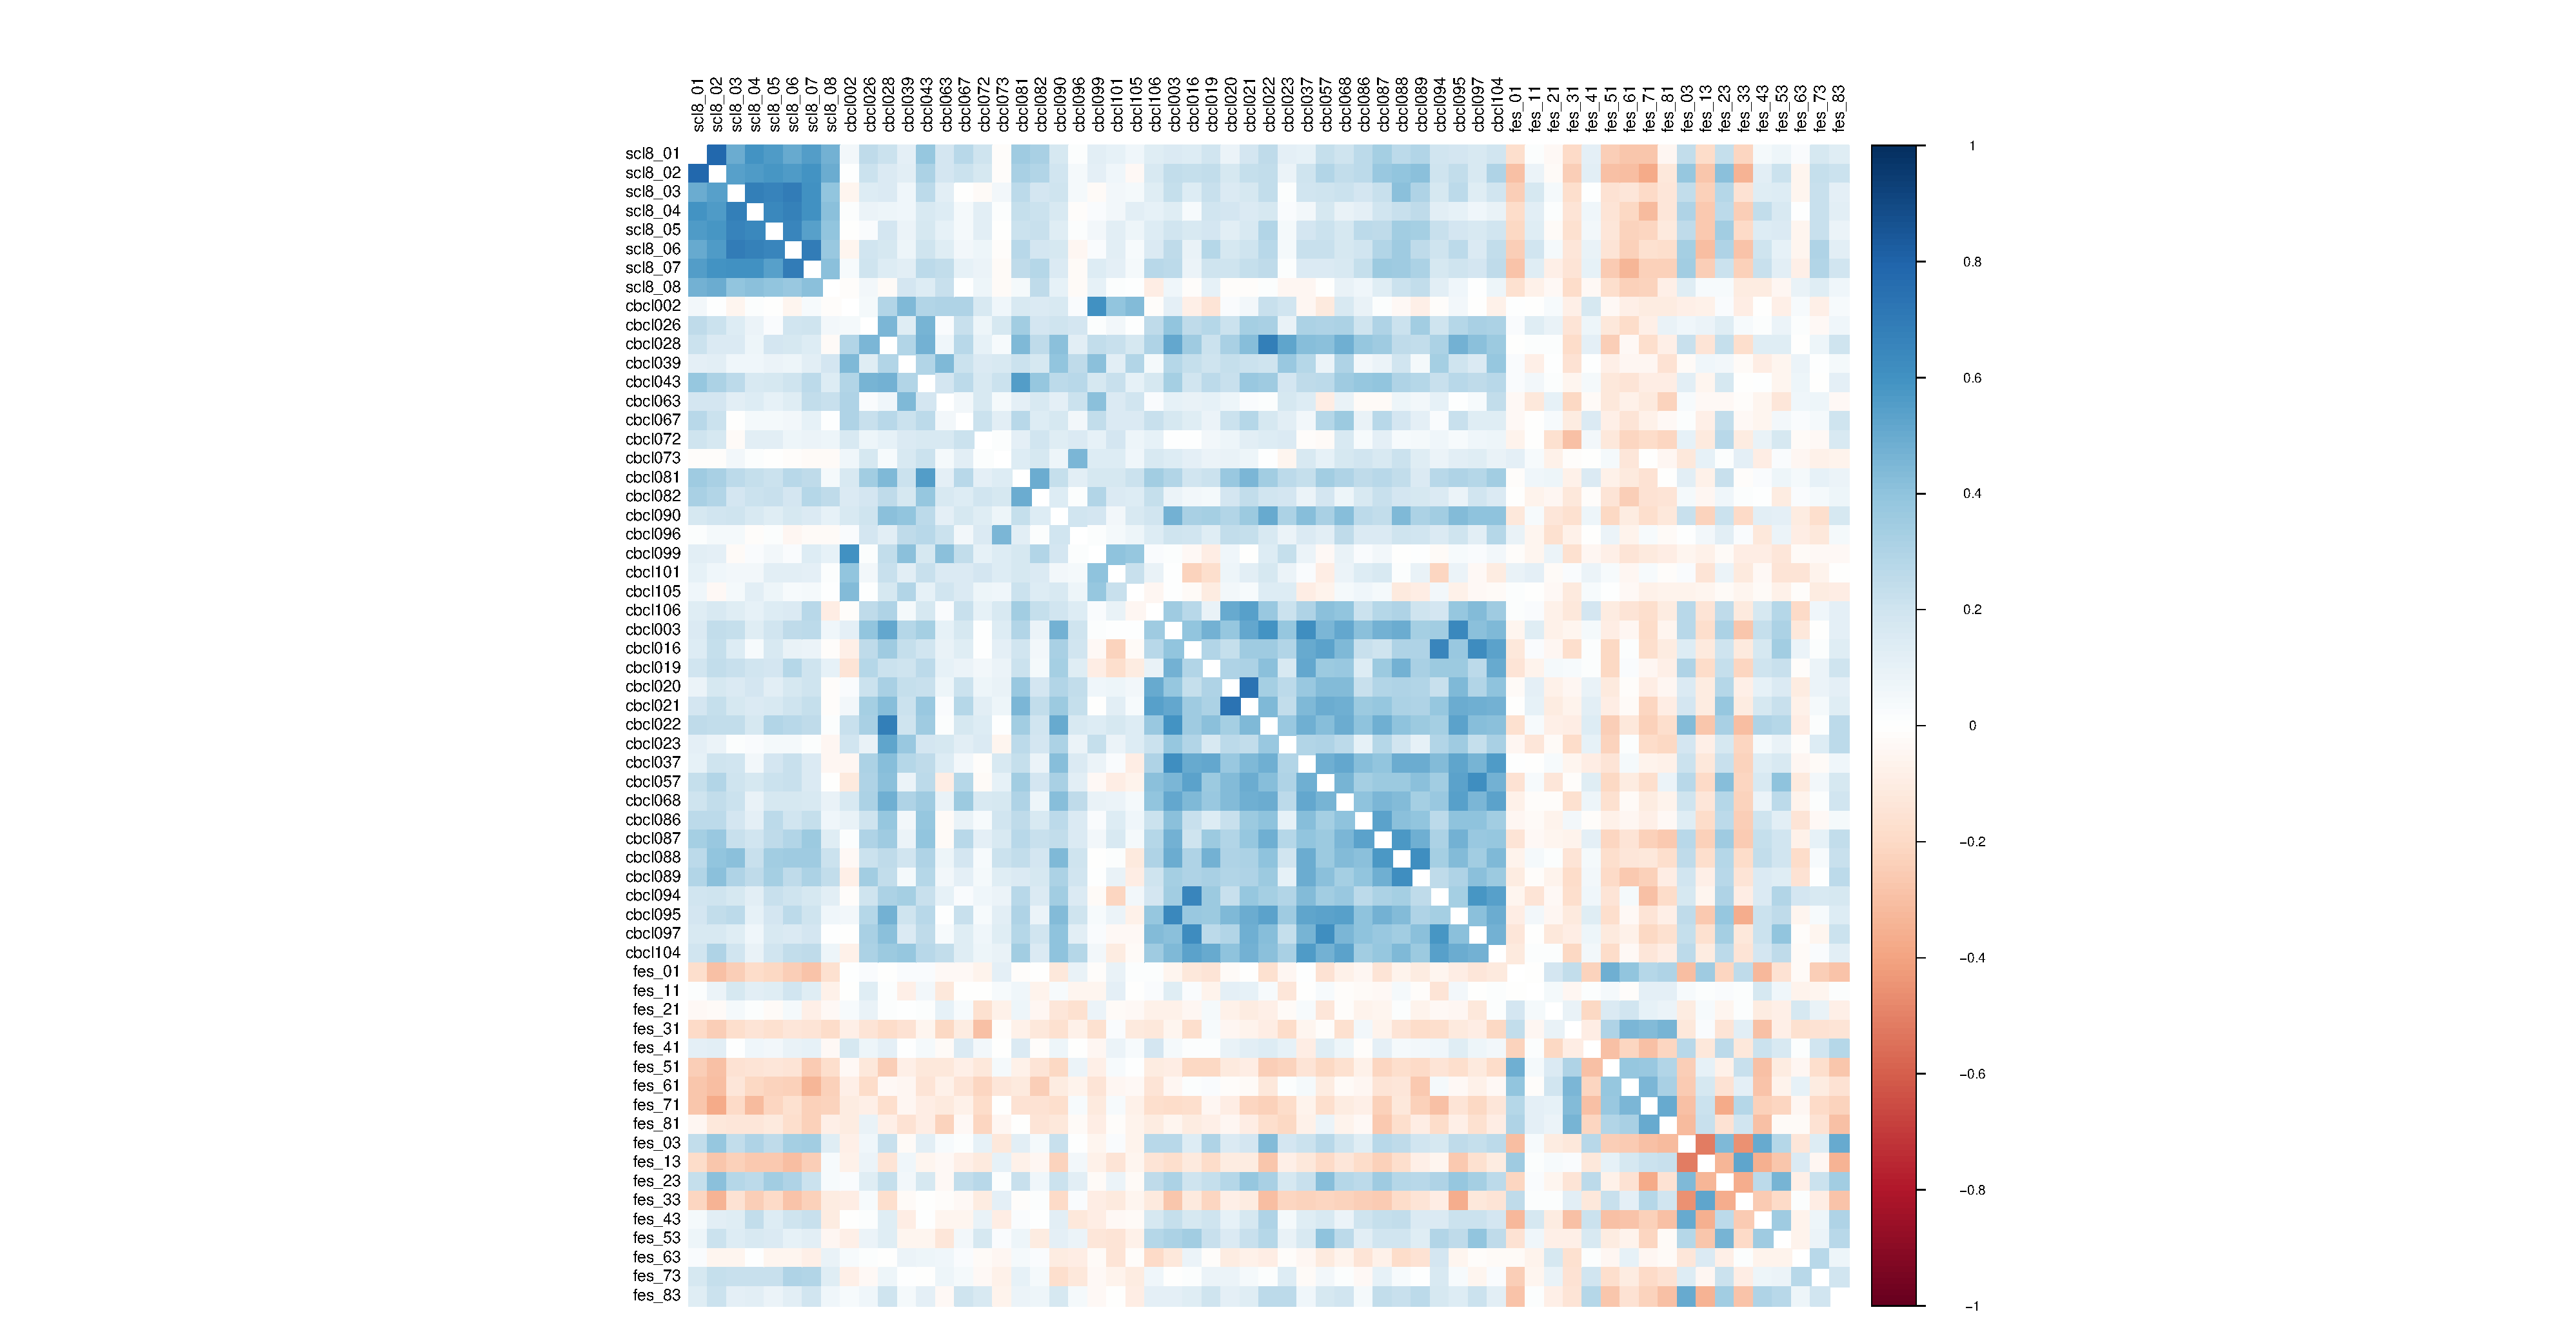
\includegraphics[width=\textwidth]{./Figures/heat_map.pdf}
\end{figure}

\subsection{Measurement Models of Parental Mental Health (PMH)}

\subsection{Measurement Models of Family Conflict (CON)}

\subsection{Measurement Models of Family Cohesion (COH)}

\subsection{Measurement Models of Adolescent Antisocial Behavior (ASB)}

\subsubsection{Rule-breaking Behavior (RBB)}

\subsubsection{Aggression (AGG)}


%\section{Analysis Code}\label{app:code}

\subsection{\textsf{Mplus} Script for Descriptive Statistics}

\begin{singlespacing}
    \lstinputlisting[language=Mplus,style=vscodeMplus]{Mplus/des_0.out}
\end{singlespacing}
\newpage

\subsection{\textsf{Mplus} Script for Exploratory Factor Analysis}

\begin{singlespacing}
    \lstinputlisting[language=Mplus,style=vscodeMplus]{Mplus/efa_1_pmh.out}
\end{singlespacing}

\begin{singlespacing}
    \lstinputlisting[language=Mplus,style=vscodeMplus]{Mplus/efa_2_rbb.out}
\end{singlespacing}

\newpage

\begin{singlespacing}
    \lstinputlisting[language=Mplus,style=vscodeMplus]{Mplus/efa_3_agg.out}
\end{singlespacing}

\newpage

\begin{singlespacing}
    \lstinputlisting[language=Mplus,style=vscodeMplus]{Mplus/efa_4_coh.out}
\end{singlespacing}

\newpage

\begin{singlespacing}
    \lstinputlisting[language=Mplus,style=vscodeMplus]{Mplus/efa_5_con.out}
\end{singlespacing}

\newpage

\begin{singlespacing}
    \lstinputlisting[language=Mplus,style=vscodeMplus]{Mplus/efa_6_asb.out}
\end{singlespacing}

\newpage

\subsection{\textsf{Mplus} Script for Path Analyses and SEM}

\begin{singlespacing}
    \lstinputlisting[language=Mplus,style=vscodeMplus]{Mplus/pat_0_mlr_dir.out}
\end{singlespacing}

\newpage

\begin{singlespacing}
    \lstinputlisting[language=Mplus,style=vscodeMplus]{Mplus/pat_1_mlr_med.out}
\end{singlespacing}

\newpage

\begin{singlespacing}
    \lstinputlisting[language=Mplus,style=vscodeMplus]{Mplus/sem_2_bayes_2_theory.out}
\end{singlespacing}

\newpage

\begin{singlespacing}
    \lstinputlisting[language=Mplus,style=vscodeMplus]{Mplus/sem_3_bayes_2_free.out}
\end{singlespacing}

\newpage

\begin{singlespacing}
    \lstinputlisting[language=Mplus,style=vscodeMplus]{Mplus/sem_4_bayes_6_free.out}
\end{singlespacing}

\end{document}
